\chapter{A \textit{ISA RISC-V}}\label{CapISA}

% Resumo opcional. Comentar se não usar.
%\resumodocapitulo{Resumo opcional}

    \section{Visão Geral da Arquitetura}

        {A \textit{ISA RISC-V} é uma arquitetura modular, sendo o módulo base de operações com inteiros mandatório em qualquer implementação. Os demais módulos são extensões de uso opcional. A arquitetura não suporta \textit{branch delay slots} e aceita instruções de tamanho variável. A codificação das instruções de tamanho variável é mostrada na Figura~\ref{fig:riscv_var_length}. As instruções presentes no módulo base correspondem ao mínimo necessário para emular por \textit{software} as demais extensões (com exceção das operações atômicas).}

        \begin{figure}[H]
        \centering
            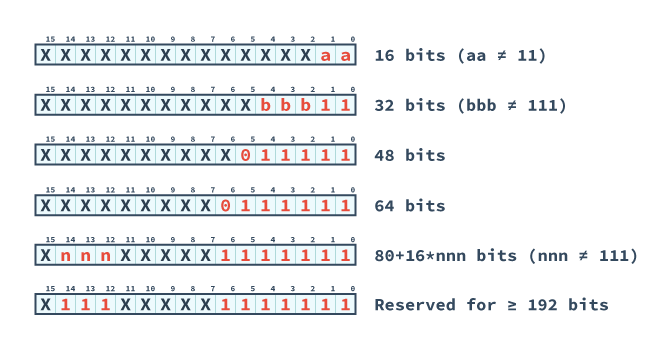
\includegraphics[width=1\linewidth]{figs/RV_InstructionLength.png}
            \caption{Codificação de instruções de tamanho variável da arquitetura \textit{RISC-V}.}\label{fig:riscv_var_length}
        \end{figure}

        \clearpage

        {A nomenclatura do conjunto de instruções implementado segue a seguinte estrutura:}

        \begin{itemize}[leftmargin=20mm]
            \item {As letras ``RV'';}
            \item {A largura dos registradores do módulo Inteiro;}
            \item {A letra ``I'' representando a base Inteira. Caso o subconjunto Embarcado (\textit{Embedded}) seja implementado, substitui-se pela letra ``E'';}
            \item {Demais letras identificadoras de módulos opcionais.}
        \end{itemize}

        {Assim, uma implementação com registradores de 64 bits somente com o módulo base de Inteiros é denominado ``RV64I''.}


        \section{Módulo Inteiro}

            {}


        \section{Extensões}

            \subsection{Extensão M}

                {}


            \subsection{Extensão A}

                {}


            \subsection{Extensão F}

                {}


            \subsection{Extensão D}

                {}


            \subsection{Outras Extensões}

                {}

    \section{Arquitetura Privilegiada}

        {}


    \section{Formatos de Instruções}

        \begin{figure}[H]
        \centering
            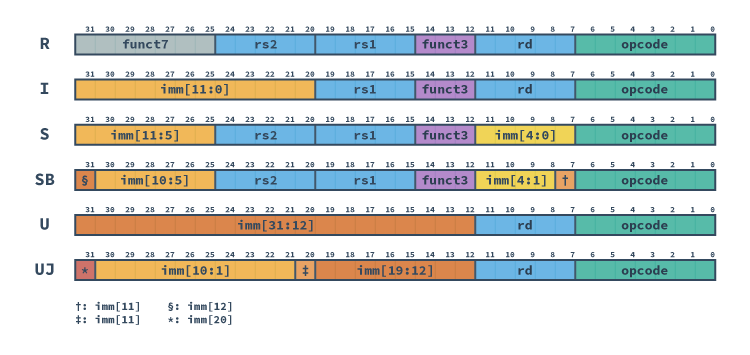
\includegraphics[width=1\linewidth]{figs/RV_Formats.png}
            \caption{Formatos de Instruções da \textit{ISA RISC-V}.}\label{fig:riscv_formats}
        \end{figure}


        % \begin{figure}[H]
        % \centering
        %     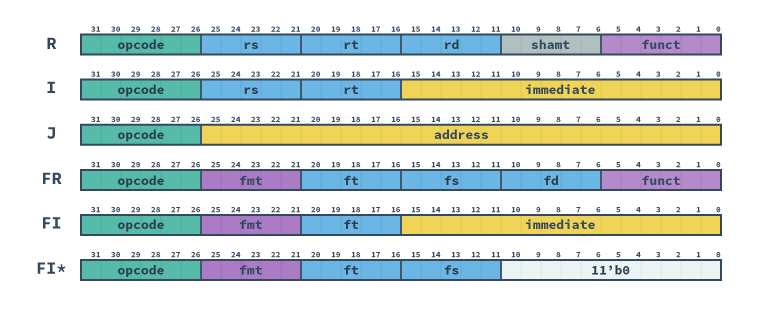
\includegraphics[width=1\linewidth]{figs/MIPS_Formats.png}
        %     \caption{Formatos de Instruções da \textit{ISA MIPS32}.}\label{fig:mips_formats}
        % \end{figure}


    \section{Formatos de Imediatos}

        \begin{figure}[H]
        \centering
            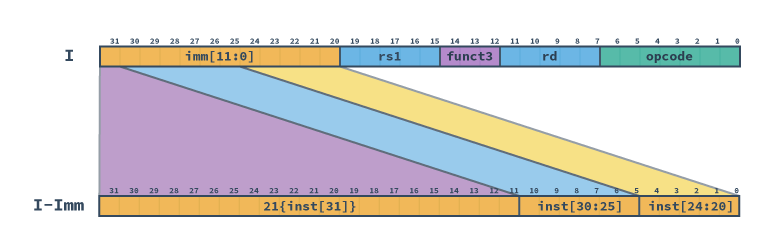
\includegraphics[width=1\linewidth]{figs/RV_I_Imm.png}
            \caption{Formação do Imediato de tipo I.}\label{fig:riscv_i_imm}
        \end{figure}

        \begin{figure}[H]
        \centering
            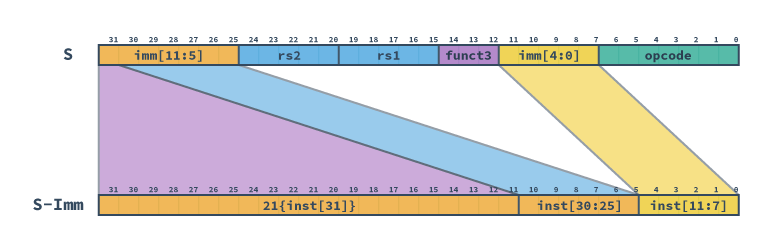
\includegraphics[width=1\linewidth]{figs/RV_S_Imm.png}
            \caption{Formação do Imediato de tipo S.}\label{fig:riscv_s_imm}
        \end{figure}

        \begin{figure}[H]
        \centering
            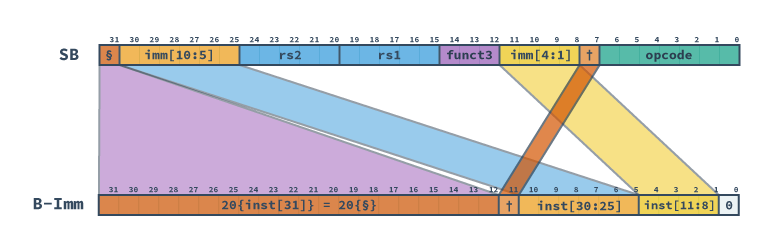
\includegraphics[width=1\linewidth]{figs/RV_B_Imm.png}
            \caption{Formação do Imediato de tipo B.}\label{fig:riscv_b_imm}
        \end{figure}

        \begin{figure}[H]
        \centering
            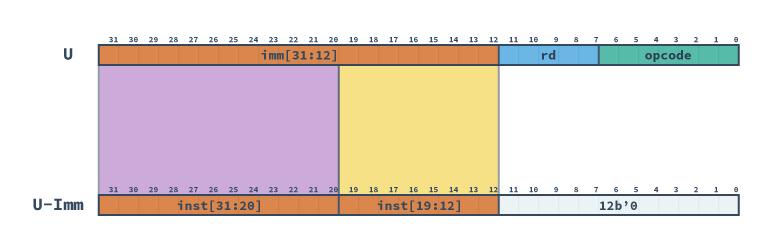
\includegraphics[width=1\linewidth]{figs/RV_U_Imm.png}
            \caption{Formação do Imediato de tipo U.}\label{fig:riscv_u_imm}
        \end{figure}

        \begin{figure}[H]
        \centering
            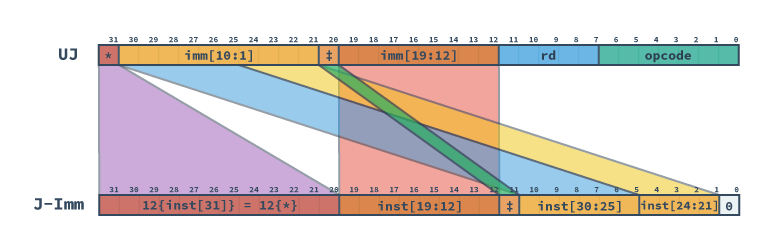
\includegraphics[width=1\linewidth]{figs/RV_J_Imm.png}
            \caption{Formação do Imediato de tipo J.}\label{fig:riscv_j_imm}
        \end{figure}


        % \begin{figure}[H]
        % \centering
        %     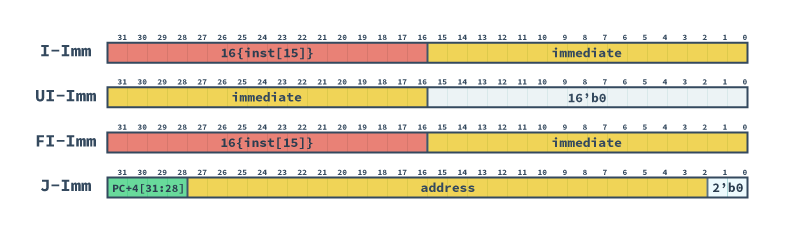
\includegraphics[width=1\linewidth]{figs/MIPS_Immediates.png}
        %     \caption{Formatos de Imediato da \textit{ISA MIPS32}.}\label{fig:mips_immediates}
        % \end{figure}
